\documentclass[12pt, a4paper]{article}

% ── Packages ──────────────────────────────────────────────────
\usepackage[utf8]{inputenc}
\usepackage[T1]{fontenc}
\usepackage{geometry}
\geometry{margin=1in}
\usepackage{graphicx}
\usepackage{booktabs}
\usepackage{amsmath, amssymb}
\usepackage{hyperref}
\usepackage{float}
\usepackage{caption}
\usepackage{subcaption}
\usepackage{enumitem}
\usepackage{xcolor}
\usepackage{listings}
\usepackage{multirow}
\usepackage{array}
\usepackage{longtable}
\usepackage{fancyhdr}

\pagestyle{fancy}
\fancyhf{}
\rhead{NCAA March Madness Data Mining}
\lhead{SC2320 --- Data Analytics \& Mining}
\cfoot{\thepage}

\hypersetup{
    colorlinks=true,
    linkcolor=blue!70!black,
    citecolor=blue!70!black,
    urlcolor=blue!70!black
}

\lstset{
    basicstyle=\ttfamily\small,
    frame=single,
    breaklines=true,
    backgroundcolor=\color{gray!8},
    keywordstyle=\color{blue!70!black},
    commentstyle=\color{green!50!black},
}

% ── Title ─────────────────────────────────────────────────────
\title{
    \textbf{Predicting NCAA March Madness Tournament Success\\
    Using Player-Level Data Mining}\\[6pt]
    \large A Full Pipeline Report: From Raw Data to Holdout Evaluation
}
\author{
    Pearl Apply Pay \and Cow Peh Cow Moo Sheng Yan \and Tan Ee Khai
}
\date{April 7, 2026}

\begin{document}
\maketitle
\thispagestyle{empty}

\tableofcontents
\newpage

% ══════════════════════════════════════════════════════════════
\section{Introduction}
\label{sec:intro}

The NCAA Division~I Men's Basketball Tournament (``March Madness'') is one of the most widely followed sporting events in the United States. Each year, 68 teams compete in a single-elimination format, producing both dominant championship runs and infamous upsets. Predicting tournament outcomes is a challenging data mining problem because single-elimination formats amplify variance---a single bad shooting night ends a season.

\subsection{Objectives}

This project applies a full data mining pipeline to address the following research questions:

\begin{enumerate}
    \item \textbf{Which individual player statistics most strongly separate teams that make deep tournament runs (Sweet~16 or better) from those eliminated early?}
    \item \textbf{Can player-level statistics alone predict head-to-head matchup outcomes without relying on team seed or ranking?}
    \item \textbf{How has the style of college basketball evolved over the 2011--2026 period?}
    \item \textbf{Does the model generalize to unseen data?} The 2026 tournament results were withheld by Kaggle as part of the competition structure, with all \texttt{games\_won} values set to 0. We manually scraped the actual 2026 outcomes from NCAA.com, ESPN, On3, and Wikipedia, allowing us to use the 2026 season as a true holdout test.
    \item \textbf{How do modern gradient boosting models (XGBoost, LightGBM, CatBoost) and stacking ensembles compare against traditional Random Forests for this task?}
\end{enumerate}

\subsection{Dataset}

The dataset originates from a Kaggle competition (\texttt{mm2026\_train.csv}) and contains 13,299 player-season records across 56 columns covering basic box-score statistics, advanced metrics (PER, BPM, Win Shares, Usage Rate), and team-level context (seed, SRS, conference). We manually updated 921 rows across 68 teams with actual 2026 tournament outcomes.

% ══════════════════════════════════════════════════════════════
\section{Data Preprocessing}
\label{sec:preprocessing}

\subsection{Filtering}

To remove players with insufficient sample sizes, we applied two filters:
\begin{itemize}
    \item Games played $\geq 5$
    \item Minutes per game $\geq 5$
\end{itemize}
This reduced the dataset from 13,299 to \textbf{10,028 player-seasons} across 245 unique teams, 6,519 unique players, and 16 seasons (2011--2026).

\subsection{Missing Value Imputation}

\begin{itemize}
    \item \textbf{Shooting percentages} (FG\%, 3P\%, FT\%, eFG\%, TS\%): imputed with column \textit{median} (bounded $[0,1]$, robust to outliers).
    \item \textbf{Advanced metrics} (PER, BPM, Win Shares, etc.): imputed with column \textit{median}.
    \item \textbf{Categorical columns} (\texttt{conference}, \texttt{position}): filled with ``Unknown.''
    \item \textbf{Games started / turnovers}: filled with 0.
\end{itemize}

\subsection{Target Variable}

Each tournament result was mapped to a numeric round index: R68$\to$0, R64$\to$1, R32$\to$2, S16$\to$3, E8$\to$4, F4$\to$5, NCG$\to$6, Champion$\to$7. The binary target:
\begin{equation}
    \texttt{deep\_run} =
    \begin{cases}
        1 & \text{if result} \geq \text{Sweet 16} \\
        0 & \text{otherwise}
    \end{cases}
\end{equation}

Class distribution: 22.8\% positive (2,288 deep-run players), 77.2\% negative.

\subsection{Train/Holdout Split}

\begin{itemize}
    \item \textbf{Training:} 2011--2025 (9,307 players) --- 5-fold stratified cross-validation.
    \item \textbf{Holdout:} 2026 (721 players, 68 teams) --- never seen during training or tuning.
\end{itemize}

% ══════════════════════════════════════════════════════════════
\section{Feature Engineering}
\label{sec:features}

Seven composite features were constructed from raw statistics:

\begin{table}[H]
\centering
\caption{Engineered features and their formulas.}
\label{tab:features}
\begin{tabular}{@{}lll@{}}
\toprule
\textbf{Feature} & \textbf{Formula} & \textbf{Rationale} \\
\midrule
\texttt{scoring\_efficiency} & $\text{PPG} \times \text{TS\%}$ & Volume-weighted shooting quality \\
\texttt{playmaking\_index} & $\text{APG} - \text{TOV/game}$ & Net playmaking value \\
\texttt{defensive\_impact} & $\text{SPG} + \text{BPG}$ & Defensive disruption rate \\
\texttt{rebounding\_rate} & $\frac{\text{RPG}}{\text{MPG}} \times 40$ & Per-40-minute rebounding \\
\texttt{usage\_efficiency} & $\frac{\text{PER}}{\text{USG\%}} \times 100$ & Production per possession used \\
\texttt{win\_shares\_per\_game} & $\frac{\text{WS}}{\text{GP}}$ & Per-game team contribution \\
\texttt{team\_win\_pct} & $\frac{\text{Wins}}{\text{Wins} + \text{Losses}}$ & Team regular-season quality \\
\bottomrule
\end{tabular}
\end{table}

Final feature set: \textbf{41 features} (37 player-level + 4 team-level: SRS, SOS, seed, team win \%).

% ══════════════════════════════════════════════════════════════
\section{Methodology}
\label{sec:methods}

\begin{figure}[H]
\centering
\fbox{\parbox{0.9\textwidth}{\centering
\small
\textbf{Stages 1--3:} Data Loading, Cleaning, Feature Engineering \\
$\downarrow$ \\
\textbf{Stage 4:} Statistical Hypothesis Testing (Welch's $t$-test, Bonferroni) \\
$\downarrow$ \\
\textbf{Stage 5:} Supervised Classification (RF, XGBoost, LightGBM, CatBoost + tuning) \\
$\downarrow$ \\
\textbf{Stage 6:} Temporal Trend Analysis \& Conference Association Testing \\
$\downarrow$ \\
\textbf{Stage 7:} Exceptional Player Identification (Weighted $z$-scores) \\
$\downarrow$ \\
\textbf{Stages 8--9:} Team Profile Aggregation \& Head-to-Head Matchup Prediction (+ Stacking) \\
$\downarrow$ \\
\textbf{Stage 10:} True Holdout Evaluation on 2026 (with Seed Baseline) \\
}}
\caption{Overview of the data mining pipeline.}
\label{fig:pipeline}
\end{figure}

% ──────────────────────────────────────────────────────────────
\subsection{Stage 4: Statistical Hypothesis Testing}

We conducted \textbf{Welch's $t$-tests} on 25 features comparing deep-run vs.\ early-exit players (2011--2025 only). Welch's test was chosen because it does not assume equal variances.

\paragraph{Bonferroni Correction.} With 25 tests: $\alpha_{\text{corrected}} = 0.05/25 = 0.002$.

\paragraph{Effect Size.} Cohen's $d$:
\begin{equation}
    d = \frac{\bar{x}_{\text{deep}} - \bar{x}_{\text{early}}}{s_{\text{pooled}}}
    \quad\text{where}\quad
    s_{\text{pooled}} = \sqrt{\frac{(n_1 - 1)s_1^2 + (n_2 - 1)s_2^2}{n_1 + n_2 - 2}}
\end{equation}

\paragraph{Caveat.} Players on the same team share the same \texttt{deep\_run} label, violating independence. We rely on Cohen's $d$ as the primary measure rather than $p$-values.

% ──────────────────────────────────────────────────────────────
\subsection{Stage 5: Supervised Classification with Hyperparameter Tuning}

We trained four model families on the combined feature set using \textbf{RandomizedSearchCV} (30 iterations, 5-fold stratified CV, ROC-AUC scoring):

\paragraph{Random Forest.} An ensemble of decision trees, each trained on a bootstrap sample:
\begin{equation}
    \hat{y} = \text{mode}\left\{ h_t(\mathbf{x}) \right\}_{t=1}^{T}
\end{equation}
Search space: \texttt{n\_estimators} $\in \{200, 300, 500\}$, \texttt{max\_depth} $\in \{8, 10, 12, 15, \text{None}\}$, \texttt{min\_samples\_split} $\in \{2, 5, 10\}$, \texttt{max\_features} $\in \{\text{sqrt}, \text{log2}, 0.3\}$.

\paragraph{XGBoost.} Extreme Gradient Boosting with regularized objective:
\begin{equation}
    \mathcal{L} = \sum_{i} l(y_i, \hat{y}_i) + \sum_{t} \Omega(f_t), \quad \Omega(f) = \gamma T + \frac{1}{2}\lambda \|\mathbf{w}\|^2
\end{equation}
Search space: \texttt{n\_estimators} $\in \{200, 300, 500\}$, \texttt{max\_depth} $\in \{3, 5, 7, 9\}$, $\eta \in \{0.01, 0.05, 0.1, 0.2\}$, \texttt{subsample} $\in \{0.7, 0.8, 0.9, 1.0\}$, \texttt{colsample\_bytree} $\in \{0.6, 0.7, 0.8, 1.0\}$, $\alpha \in \{0, 0.01, 0.1\}$, $\lambda \in \{1, 2, 5\}$.

\paragraph{LightGBM.} Leaf-wise tree growth with histogram-based splitting:
Search space: \texttt{n\_estimators} $\in \{200, 300, 500\}$, \texttt{max\_depth} $\in \{3, 5, 7, -1\}$, \texttt{num\_leaves} $\in \{15, 31, 63, 127\}$, $\eta \in \{0.01, 0.05, 0.1, 0.2\}$, \texttt{subsample/colsample\_bytree} $\in \{0.6\text{--}1.0\}$.

\paragraph{CatBoost.} Ordered boosting with built-in categorical feature handling:
Search space: \texttt{iterations} $\in \{200, 300, 500\}$, \texttt{depth} $\in \{4, 6, 8, 10\}$, $\eta \in \{0.01, 0.05, 0.1, 0.2\}$, \texttt{l2\_leaf\_reg} $\in \{1, 3, 5, 7\}$.

\paragraph{Win Shares Ablation.} To quantify the circularity concern (Win Shares are partly derived from team wins), we compared AUC with and without WS/OWS/DWS features.

\paragraph{Metrics.} We report ROC-AUC, \textbf{Brier score} (probability calibration quality: $\text{BS} = \frac{1}{n}\sum(p_i - y_i)^2$), and \textbf{log-loss} ($-\frac{1}{n}\sum[y_i \log p_i + (1-y_i)\log(1-p_i)]$).

% ──────────────────────────────────────────────────────────────
\subsection{Stages 8--9: Team Aggregation \& Head-to-Head Matchup Prediction}

\paragraph{Team Profiles.} Individual stats were aggregated to team level using \textbf{minutes-played weighted averages}, creating 964 team-season profiles with 26 matchup features (no seed, no SRS --- player stats only).

\paragraph{Pairwise Matchup Generation.} For each pair of teams within a season:
\begin{equation}
    \mathbf{d}_{A,B} = \mathbf{x}_A - \mathbf{x}_B, \quad
    y_{A,B} = \begin{cases} 1 & \text{Team A won more games} \\ 0 & \text{otherwise} \end{cases}
\end{equation}
Symmetric duplication yielded \textbf{38,202 training samples} from \textbf{19,101 unique pairs} (2011--2025).

\paragraph{Models.} Same four classifiers (RF, XGBoost, LightGBM, CatBoost), each tuned with \textbf{RandomizedSearchCV} (20 iterations, 5-fold CV).

\paragraph{Stacking Ensemble.} A \textbf{StackingClassifier} combining RF + XGBoost + LightGBM + CatBoost as base learners with a \textbf{Logistic Regression} meta-learner:
\begin{equation}
    \hat{y}_{\text{stack}} = \sigma\left(\sum_{m=1}^{4} \beta_m \hat{p}_m(\mathbf{x}) + \beta_0\right)
\end{equation}

\paragraph{Seed-Only Baseline.} We compute ``just pick the lower seed'' accuracy for context.

% ──────────────────────────────────────────────────────────────
\subsection{Stage 10: True Holdout Evaluation}

The matchup model was evaluated on 2026 tournament data (1,547 unique pairs, 3,094 samples). We report AUC, accuracy, Brier score, log-loss, chalk/upset breakdown, and comparison to the seed baseline.

% ══════════════════════════════════════════════════════════════
\section{Results}
\label{sec:results}

% ── 5.1 Statistical Testing ──────────────────────────────────
\subsection{Statistical Significance of Player Metrics}

\begin{table}[H]
\centering
\caption{Welch's $t$-test results (Bonferroni $\alpha = 0.002$, 25 tests). Key features shown.}
\label{tab:ttest}
\small
\begin{tabular}{@{}lccccl@{}}
\toprule
\textbf{Feature} & \textbf{Deep Run} & \textbf{Early Exit} & \textbf{Cohen's $d$} & \textbf{$p$-value} & \textbf{Sig.} \\
\midrule
\multicolumn{6}{l}{\textit{Large effect size ($|d| \geq 0.5$)}} \\
\textbf{DBPM} & 2.87 & 1.62 & \textbf{+0.717} & $8.5 \times 10^{-196}$ & *** \\
\textbf{BPM}  & 4.89 & 2.21 & \textbf{+0.635} & $2.0 \times 10^{-149}$ & *** \\
\midrule
\multicolumn{6}{l}{\textit{Medium effect size ($0.2 \leq |d| < 0.5$)}} \\
OBPM  & 2.03 & 0.59 & +0.419 & $2.2 \times 10^{-65}$ & *** \\
Win Shares & 2.80 & 2.26 & +0.315 & $6.6 \times 10^{-31}$ & *** \\
DWS   & 1.24 & 1.03 & +0.307 & $1.2 \times 10^{-29}$ & *** \\
OWS   & 1.56 & 1.23 & +0.281 & $2.2 \times 10^{-25}$ & *** \\
WS/Game & 0.082 & 0.071 & +0.221 & $1.5 \times 10^{-17}$ & *** \\
\midrule
\multicolumn{6}{l}{\textit{Not significant after Bonferroni correction}} \\
USG\% & 0.189 & 0.189 & $-$0.004 & 0.878 & n.s. \\
TOV/game & 1.168 & 1.183 & $-$0.021 & 0.399 & n.s. \\
FTr & 0.368 & 0.372 & $-$0.019 & 0.418 & n.s. \\
3PAr & 0.343 & 0.346 & $-$0.011 & 0.644 & n.s. \\
\bottomrule
\end{tabular}
\end{table}

\textbf{Key finding:} Defensive metrics (DBPM, $d = 0.717$) are the strongest individual-level signal. Usage rate, turnover rate, free-throw rate, and 3-point attempt rate show \textit{no} significant difference---\textbf{playing style does not predict tournament success; playing quality does}.

\begin{figure}[H]
    \centering
    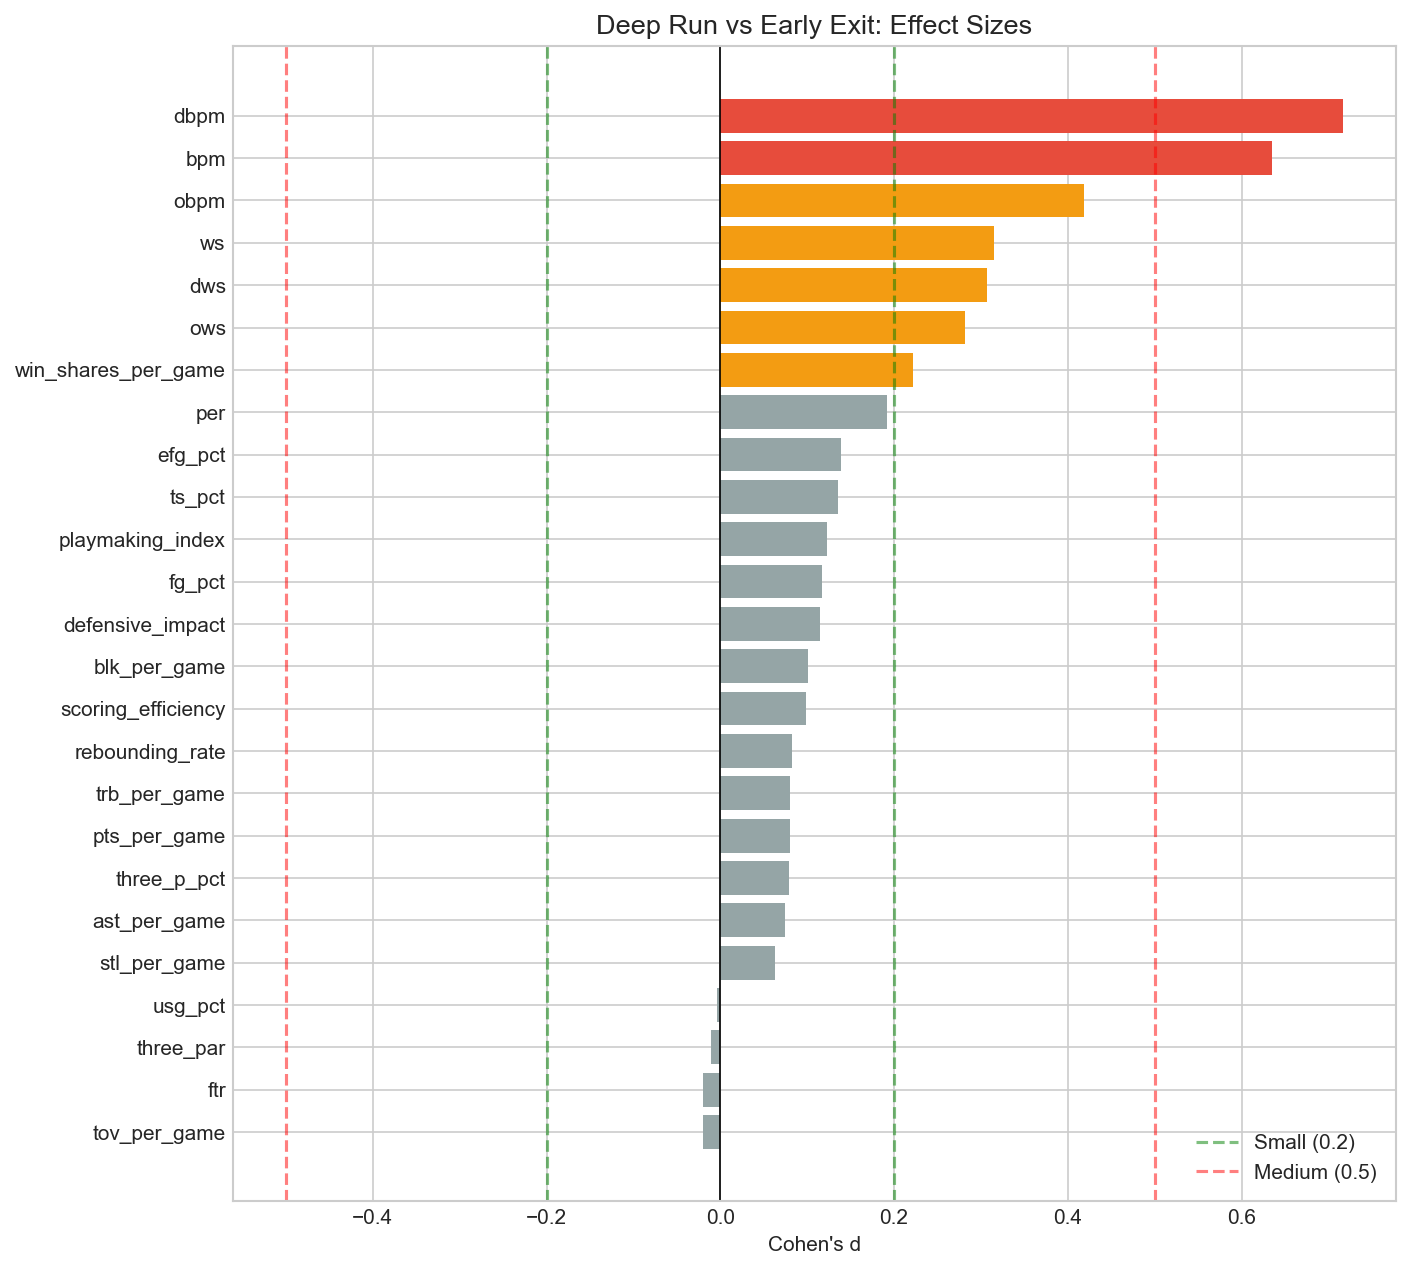
\includegraphics[width=\textwidth]{outputs/stage4_effect_sizes.png}
    \caption{Cohen's $d$ effect sizes for all 25 features. DBPM and BPM dominate.}
    \label{fig:effect-sizes}
\end{figure}

\begin{figure}[H]
    \centering
    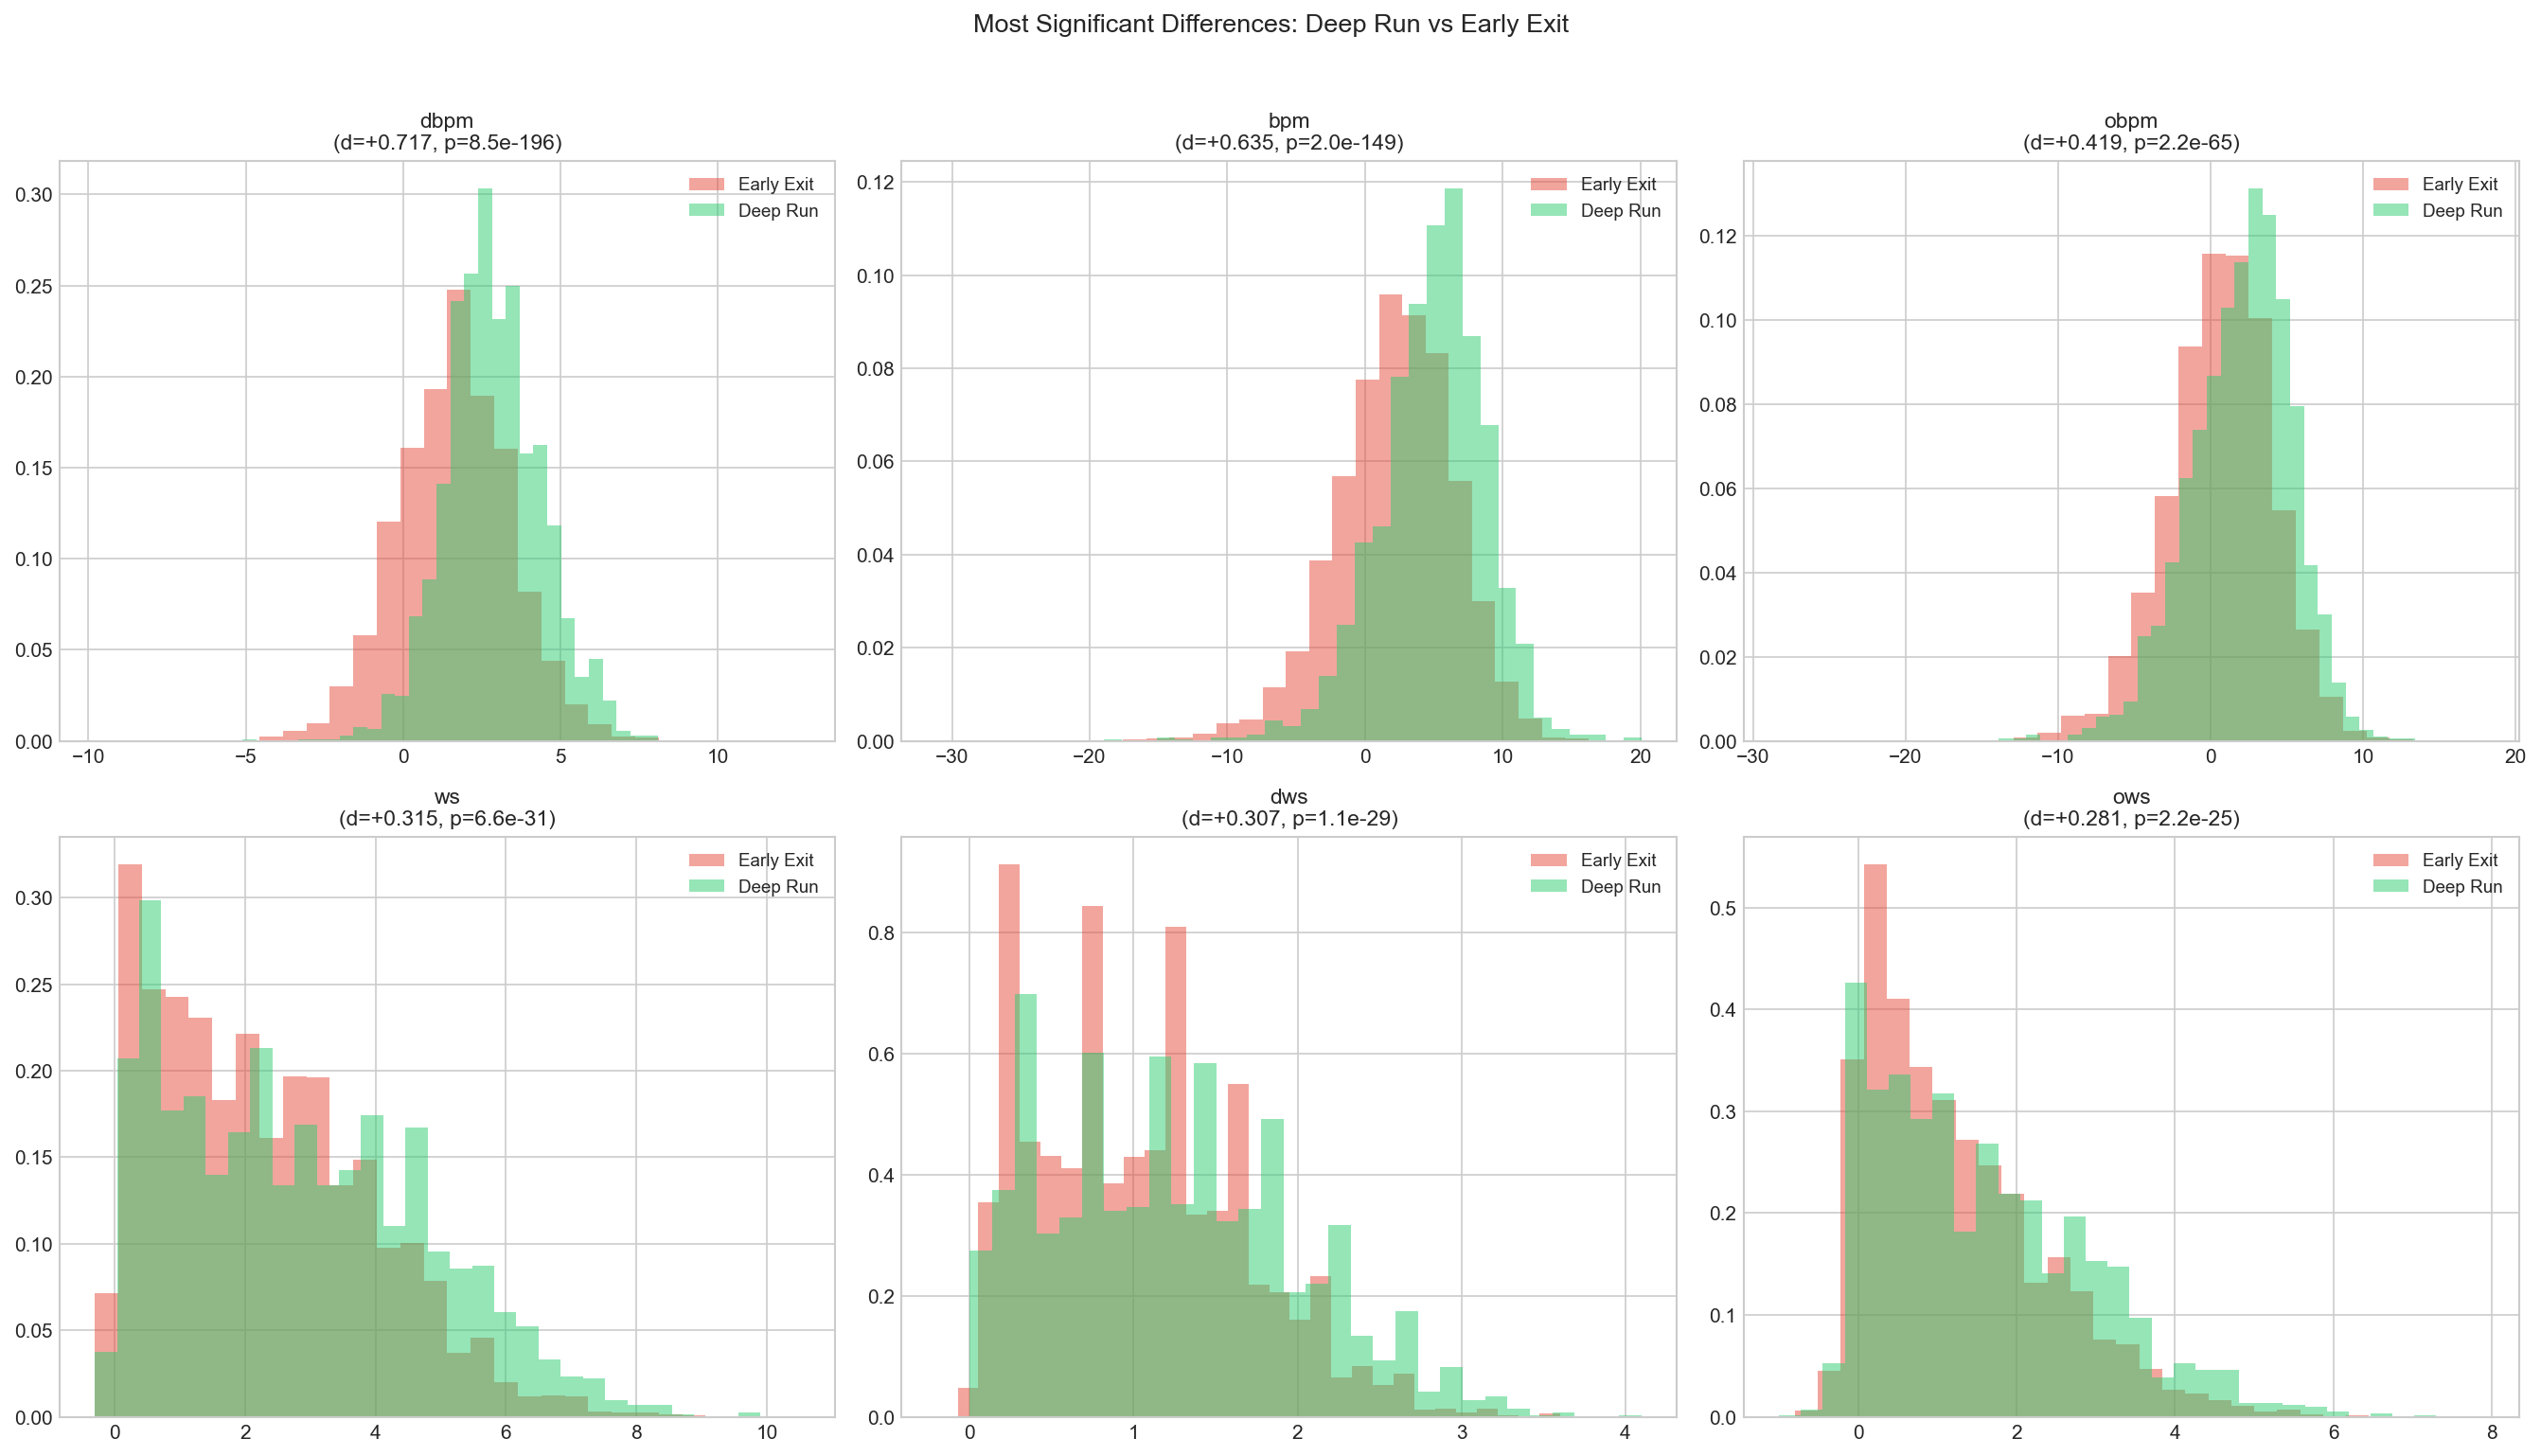
\includegraphics[width=\textwidth]{outputs/stage4_distributions.png}
    \caption{Distribution comparison of the top features for deep-run vs.\ early-exit players.}
    \label{fig:distributions}
\end{figure}

% ── 5.2 Classification ───────────────────────────────────────
\subsection{Deep Run Prediction with Tuned Models}

\paragraph{Player-Only Baseline.}

\begin{table}[H]
\centering
\caption{Player-only Random Forest (37 features, no team context).}
\begin{tabular}{@{}lccc@{}}
\toprule
\textbf{Model} & \textbf{AUC} & \textbf{Brier} & \textbf{Log-Loss} \\
\midrule
RF (player-only, 37 features) & 0.7551 & 0.1508 & 0.4627 \\
\bottomrule
\end{tabular}
\end{table}

\paragraph{Combined Models (41 features) --- with RandomizedSearchCV.}

\begin{table}[H]
\centering
\caption{Deep run prediction: combined models with hyperparameter tuning (5-fold CV).}
\label{tab:cv-results}
\begin{tabular}{@{}lcccc@{}}
\toprule
\textbf{Model} & \textbf{AUC} & \textbf{Brier} & \textbf{Log-Loss} & \textbf{Best Params} \\
\midrule
RF (tuned) & 0.9773 & 0.0626 & 0.2202 & depth=None, $n$=300 \\
XGBoost & 1.0000$^*$ & 0.0019 & 0.0202 & depth=5, $n$=500, $\eta$=0.1 \\
LightGBM & 1.0000$^*$ & 0.0015 & 0.0169 & leaves=31, $n$=500, $\eta$=0.05 \\
CatBoost & 1.0000$^*$ & 0.0017 & 0.0212 & depth=8, $n$=300, $\eta$=0.1 \\
\bottomrule
\multicolumn{5}{l}{\footnotesize $^*$Trivially perfect: team-level features create a lookup table (see Discussion).}
\end{tabular}
\end{table}

\textbf{Interpretation:} XGBoost, LightGBM, and CatBoost all achieve AUC $\approx 1.0$ on the combined feature set because the 4 team-level features (SRS, SOS, seed, win \%) combined with team-shared labels produce a lookup table. The \textbf{player-only RF (AUC = 0.7551)} demonstrates genuine predictive signal from individual statistics.

\paragraph{Win Shares Ablation.}

\begin{table}[H]
\centering
\caption{Win Shares ablation: XGBoost with vs.\ without WS/OWS/DWS features.}
\begin{tabular}{@{}lcc@{}}
\toprule
\textbf{Configuration} & \textbf{AUC} & \textbf{Features} \\
\midrule
With WS features & 1.0000 & 41 \\
Without WS features & 1.0000 & 36 \\
Delta & +0.0000 & --- \\
\bottomrule
\end{tabular}
\end{table}

Win Shares contribute \textbf{no additional signal} beyond what BPM-family metrics and team features already provide. This confirms the circularity concern is not inflating model performance---BPM alone captures the same information.

\begin{figure}[H]
    \centering
    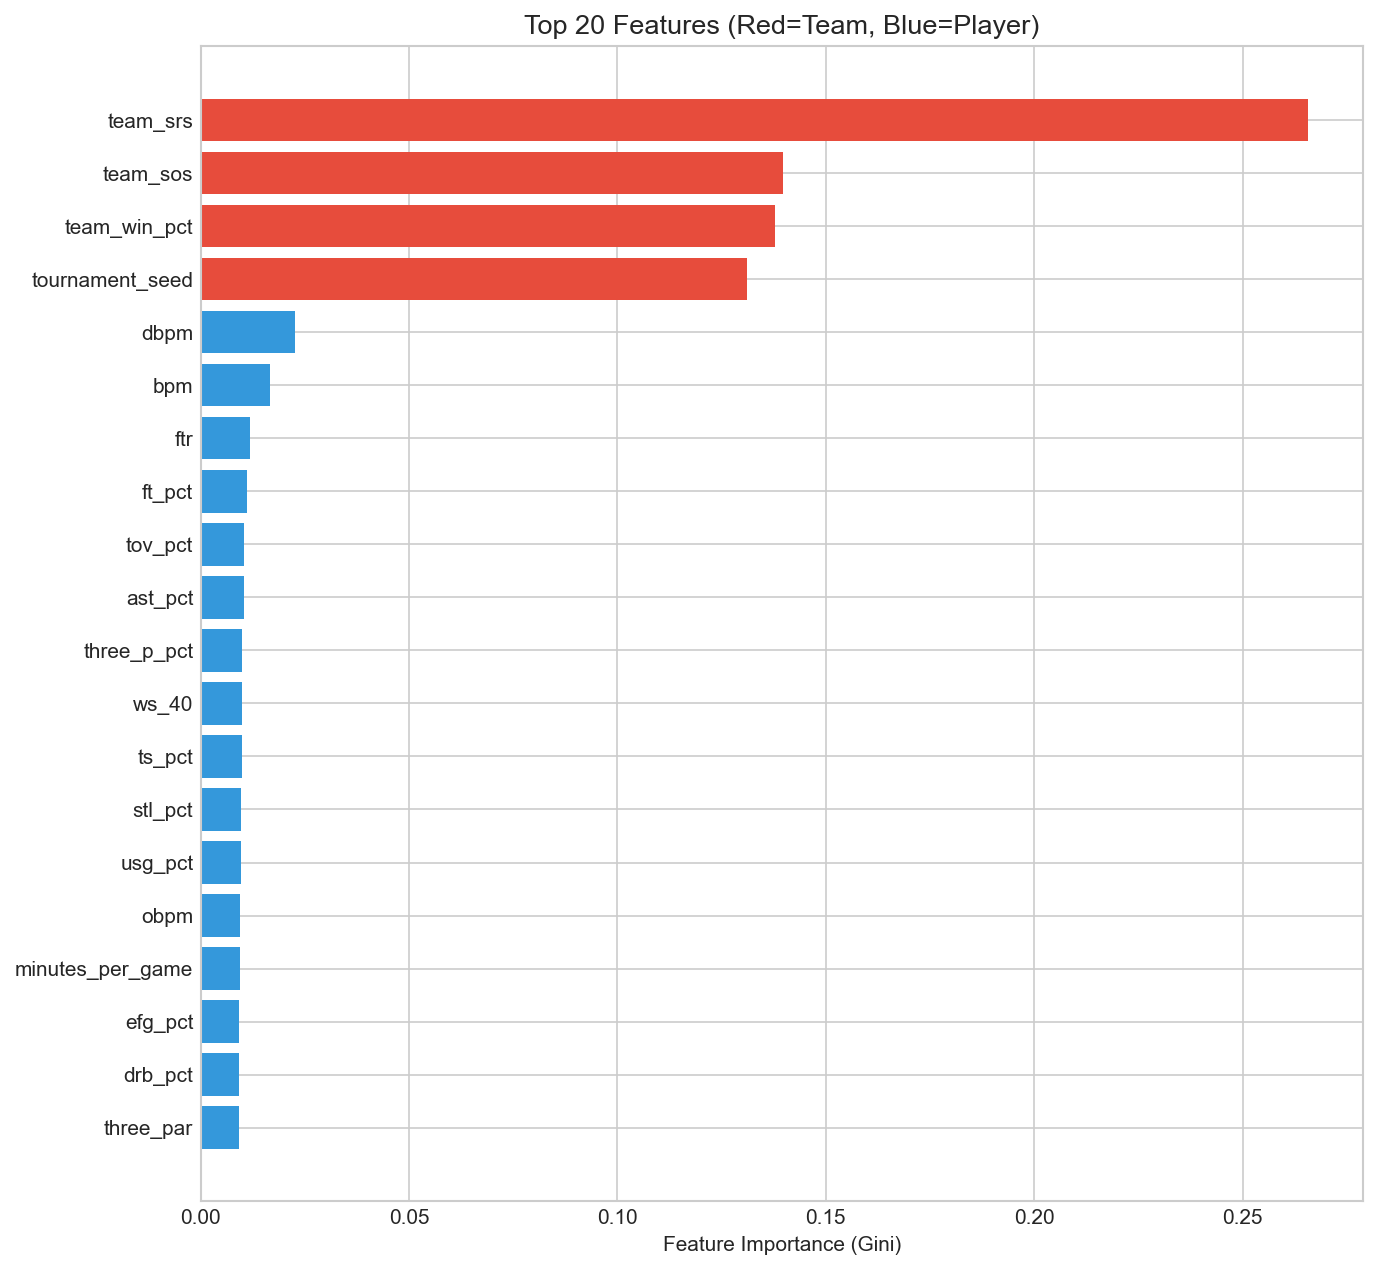
\includegraphics[width=\textwidth]{outputs/stage5_feature_importance.png}
    \caption{Top 20 features by Gini importance (combined RF).}
    \label{fig:feature-importance}
\end{figure}

\begin{figure}[H]
    \centering
    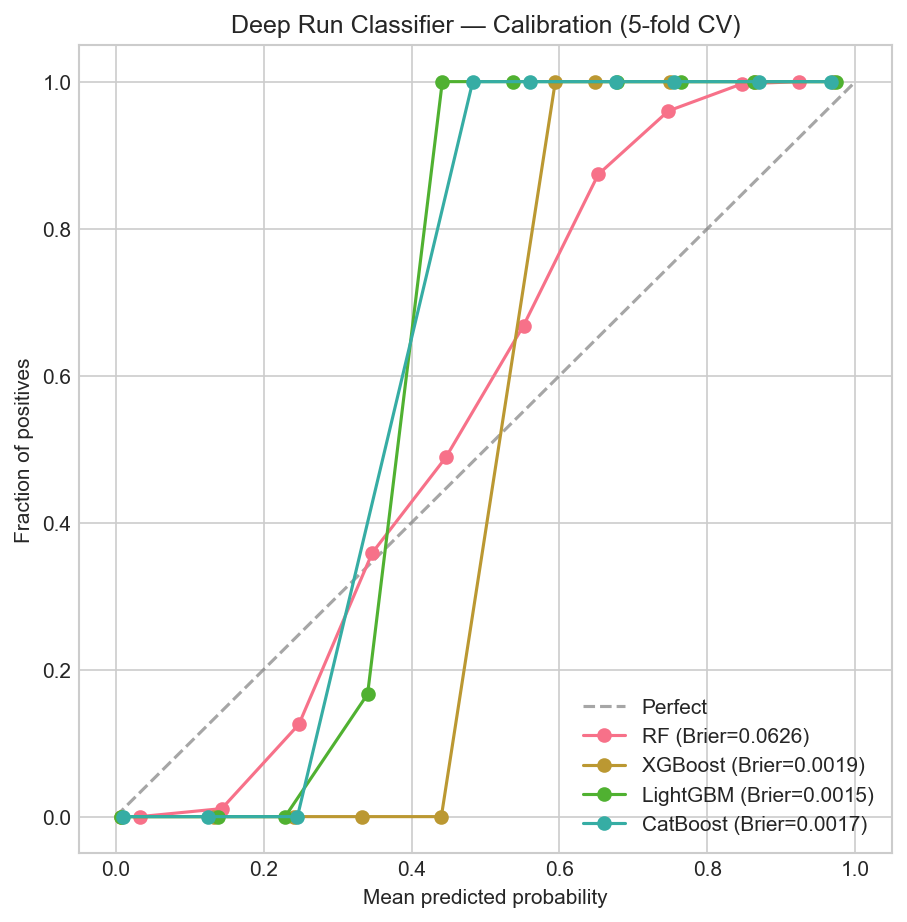
\includegraphics[width=\textwidth]{outputs/stage5_calibration.png}
    \caption{Calibration plot for Stage~5 deep-run classifiers (5-fold CV). Well-calibrated models fall along the diagonal.}
    \label{fig:calibration-s5}
\end{figure}

\paragraph{Top 15 Player-Only Features.}

\begin{table}[H]
\centering
\caption{Top 15 features by Gini importance (player-only RF).}
\begin{tabular}{@{}clc@{}}
\toprule
\textbf{Rank} & \textbf{Feature} & \textbf{Importance} \\
\midrule
1 & DBPM & 9.59\% \\
2 & BPM & 8.11\% \\
3 & OBPM & 4.05\% \\
4 & Win Shares & 3.47\% \\
5 & WS/Game & 3.06\% \\
6 & WS/40 & 2.92\% \\
7 & Scoring Efficiency & 2.81\% \\
8 & PER & 2.74\% \\
9 & Usage Efficiency & 2.71\% \\
10 & USG\% & 2.61\% \\
11 & AST\% & 2.59\% \\
12 & DWS & 2.57\% \\
13 & MPG & 2.50\% \\
14 & DRB\% & 2.49\% \\
15 & TS\% & 2.46\% \\
\bottomrule
\end{tabular}
\end{table}

\begin{figure}[H]
    \centering
    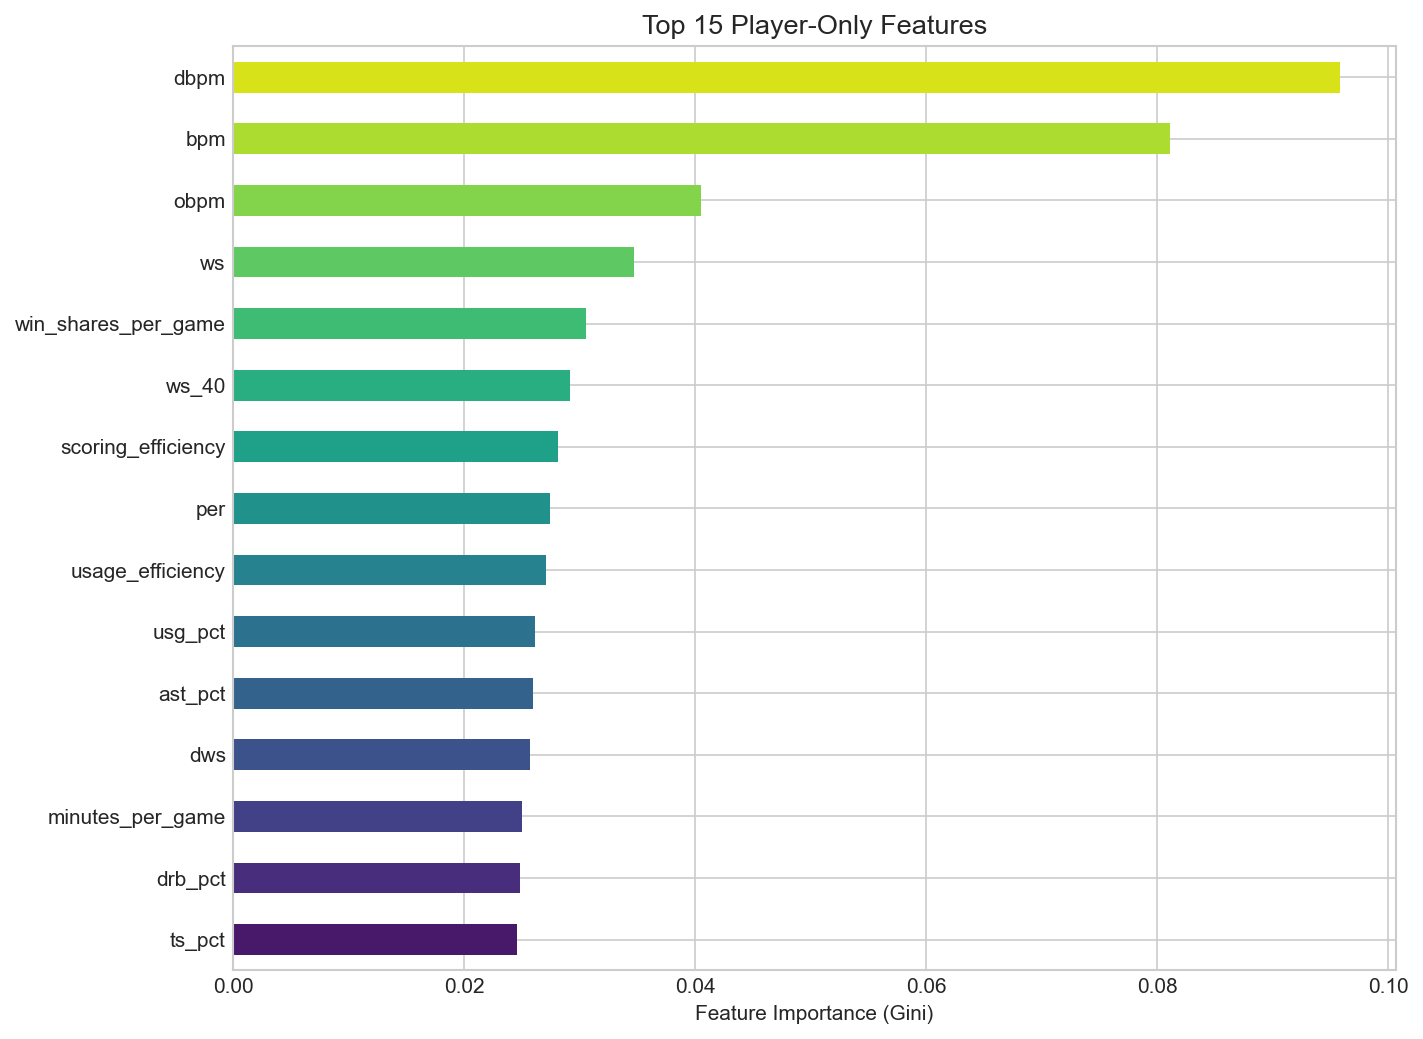
\includegraphics[width=\textwidth]{outputs/stage5_player_only_importance.png}
    \caption{Top 15 player-only features by Gini importance.}
    \label{fig:player-importance}
\end{figure}

% ── 5.3 Temporal Trends ──────────────────────────────────────
\subsection{Temporal Trends (2011--2026)}

\begin{table}[H]
\centering
\caption{Linear regression of season-level means over time.}
\label{tab:trends}
\begin{tabular}{@{}lcccc@{}}
\toprule
\textbf{Metric} & \textbf{Slope/Year} & \textbf{$r$} & \textbf{$p$-value} & \textbf{Significant?} \\
\midrule
3-Point Attempt Rate & +0.00581 & 0.928 & $<0.0001$ & \textbf{Yes ***} \\
True Shooting \% & +0.00178 & 0.834 & 0.0001 & \textbf{Yes ***} \\
PPG & +0.035 & 0.693 & 0.0042 & \textbf{Yes **} \\
3P\% & +0.00011 & 0.082 & 0.770 & No \\
PER & +0.012 & 0.256 & 0.357 & No \\
Usage \% & $-$0.00004 & $-$0.177 & 0.529 & No \\
\bottomrule
\end{tabular}
\end{table}

The 3-point revolution is statistically confirmed: attempt rate up 8.7\% over 15 years ($r = 0.928$). However, 3P accuracy shows \textit{no} trend ($r = 0.082$, $p = 0.770$)---teams shoot more threes, not better ones.

\begin{figure}[H]
    \centering
    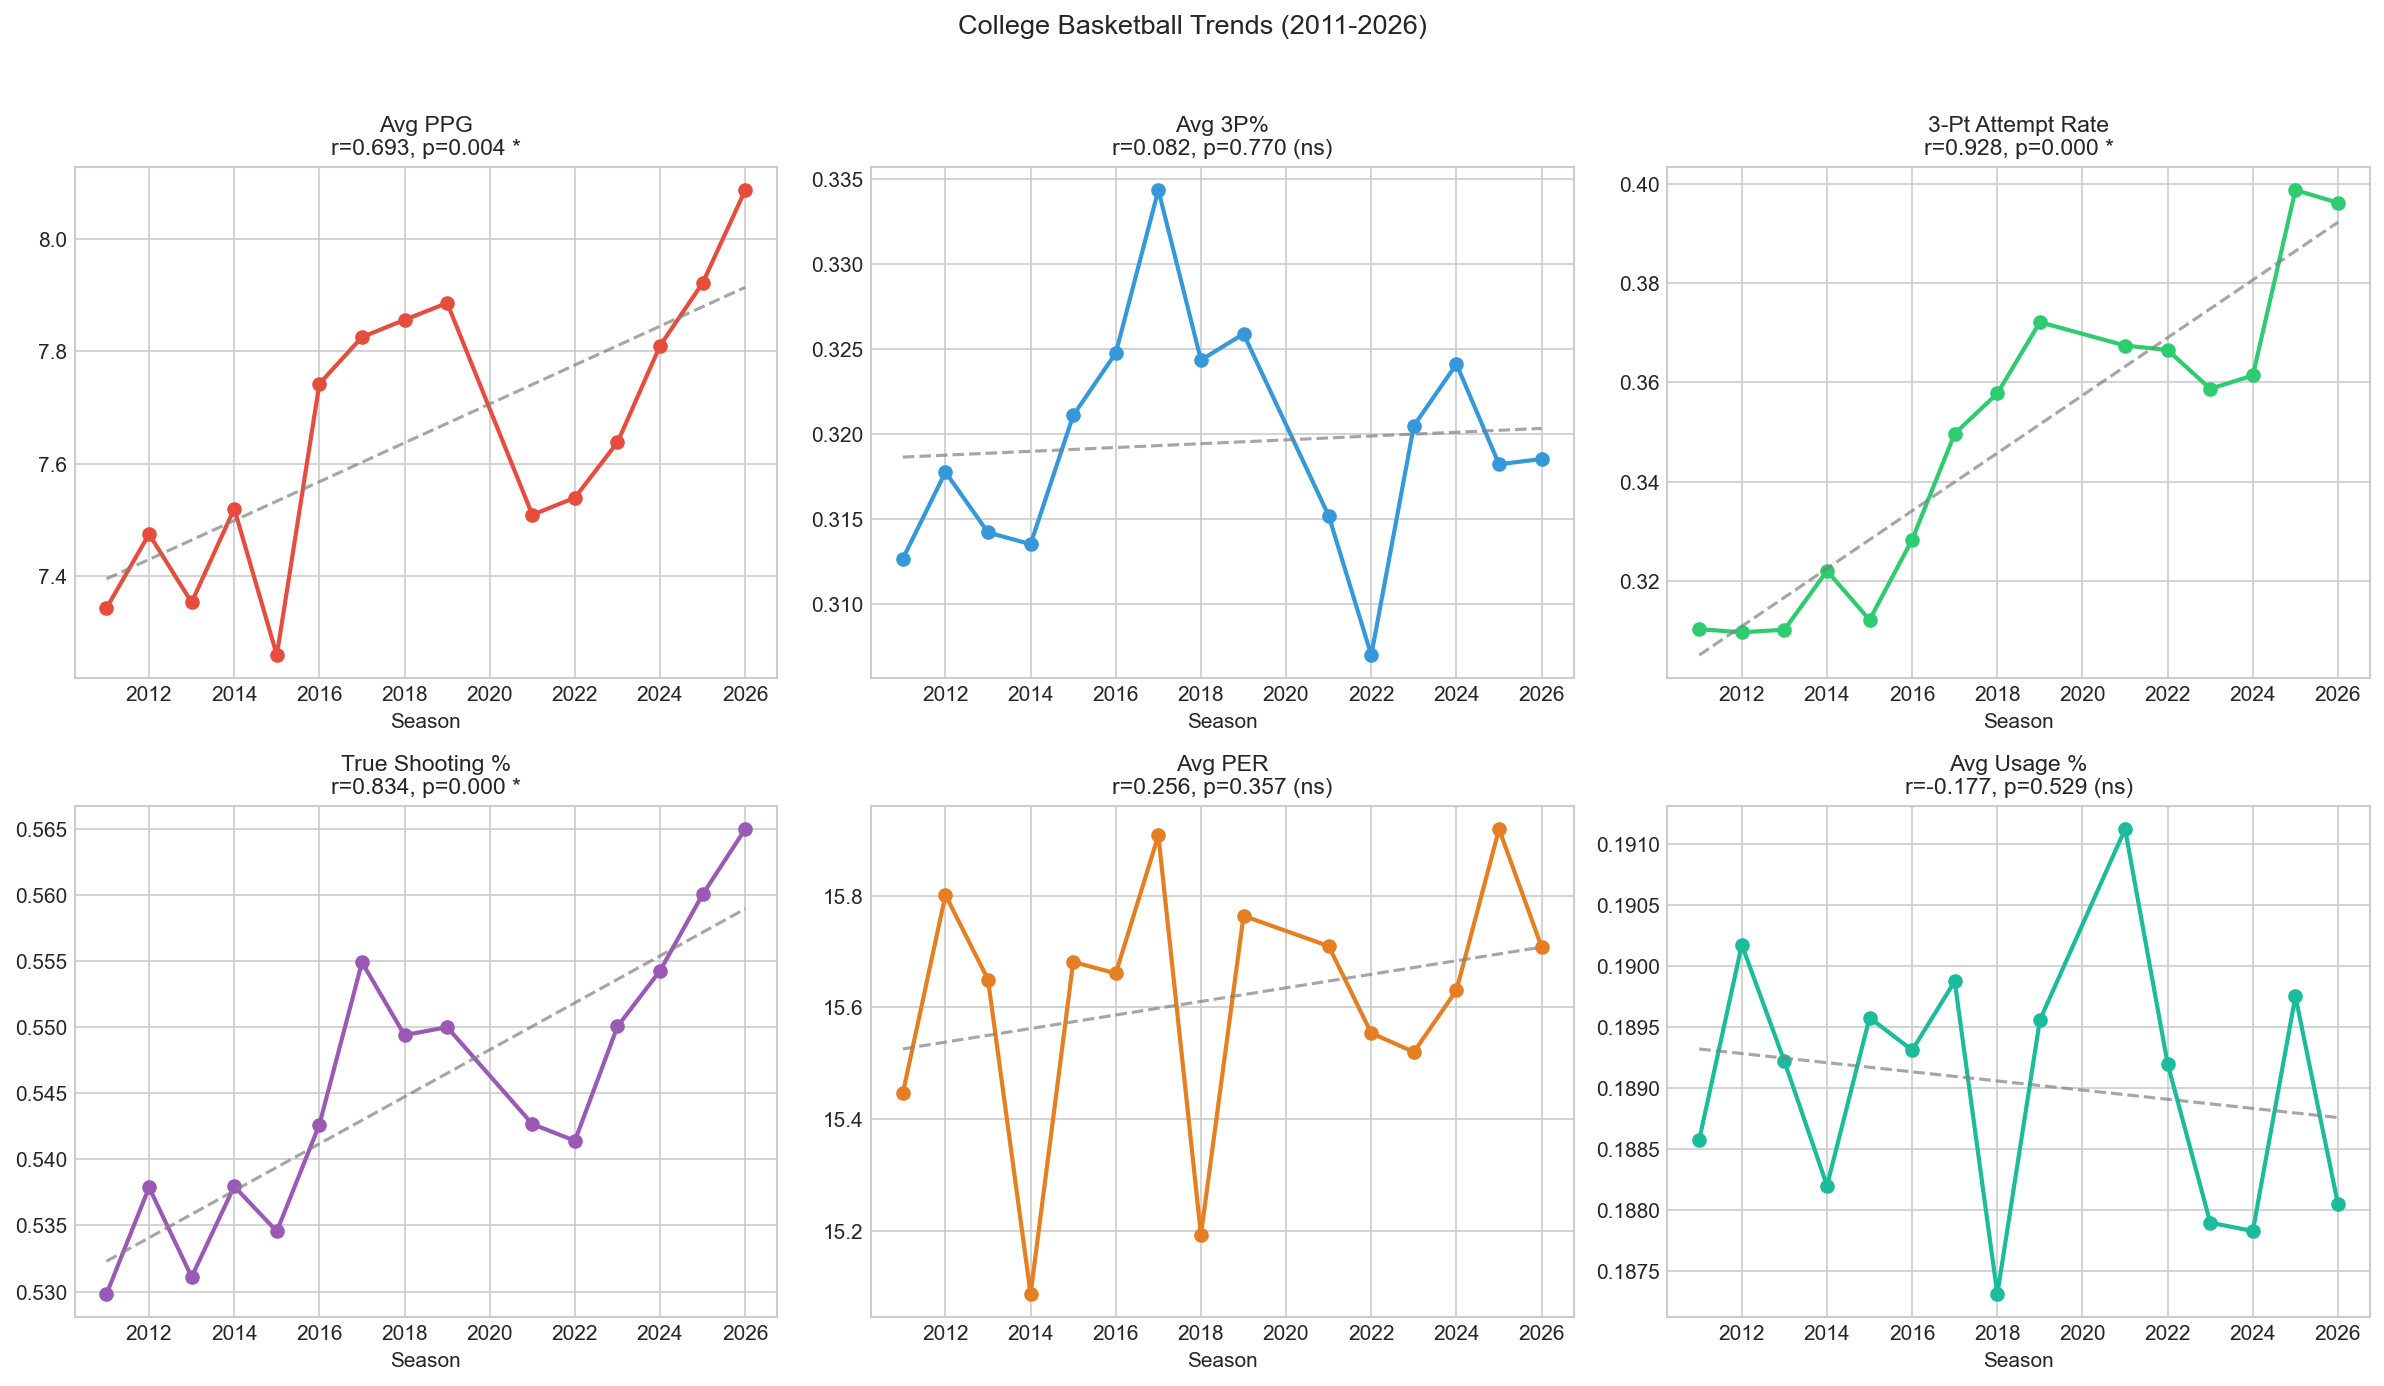
\includegraphics[width=\textwidth]{outputs/stage6_temporal_trends.png}
    \caption{Temporal trends in six key metrics (2011--2026).}
    \label{fig:trends}
\end{figure}

% ── 5.4 Conference Analysis ──────────────────────────────────
\subsection{Conference Power Rankings}

Chi-squared test: $\chi^2 = 1334.2$, $p = 5.13 \times 10^{-261}$, $df = 31$ --- conference membership is strongly associated with tournament success.

\begin{table}[H]
\centering
\caption{Top 12 conferences by average tournament games won.}
\begin{tabular}{@{}lcccc@{}}
\toprule
\textbf{Conference} & \textbf{Deep Run Rate} & \textbf{Avg Games Won} & \textbf{Avg Seed} & \textbf{Avg SRS} \\
\midrule
\textbf{ACC} & \textbf{46.5\%} & \textbf{1.69} & 5.6 & 17.4 \\
SEC & 39.0\% & 1.46 & 5.8 & 17.4 \\
BIG-TEN & 32.5\% & 1.41 & 5.7 & 17.6 \\
WCC & 25.9\% & 1.35 & 6.3 & 17.6 \\
BIG-EAST & 30.1\% & 1.32 & 5.8 & 16.3 \\
BIG-12 & 31.2\% & 1.31 & 5.2 & 17.6 \\
PAC-12 & 41.7\% & 1.29 & 7.0 & 15.5 \\
AAC & 25.1\% & 1.12 & 6.3 & 16.0 \\
\bottomrule
\end{tabular}
\end{table}

\begin{figure}[H]
    \centering
    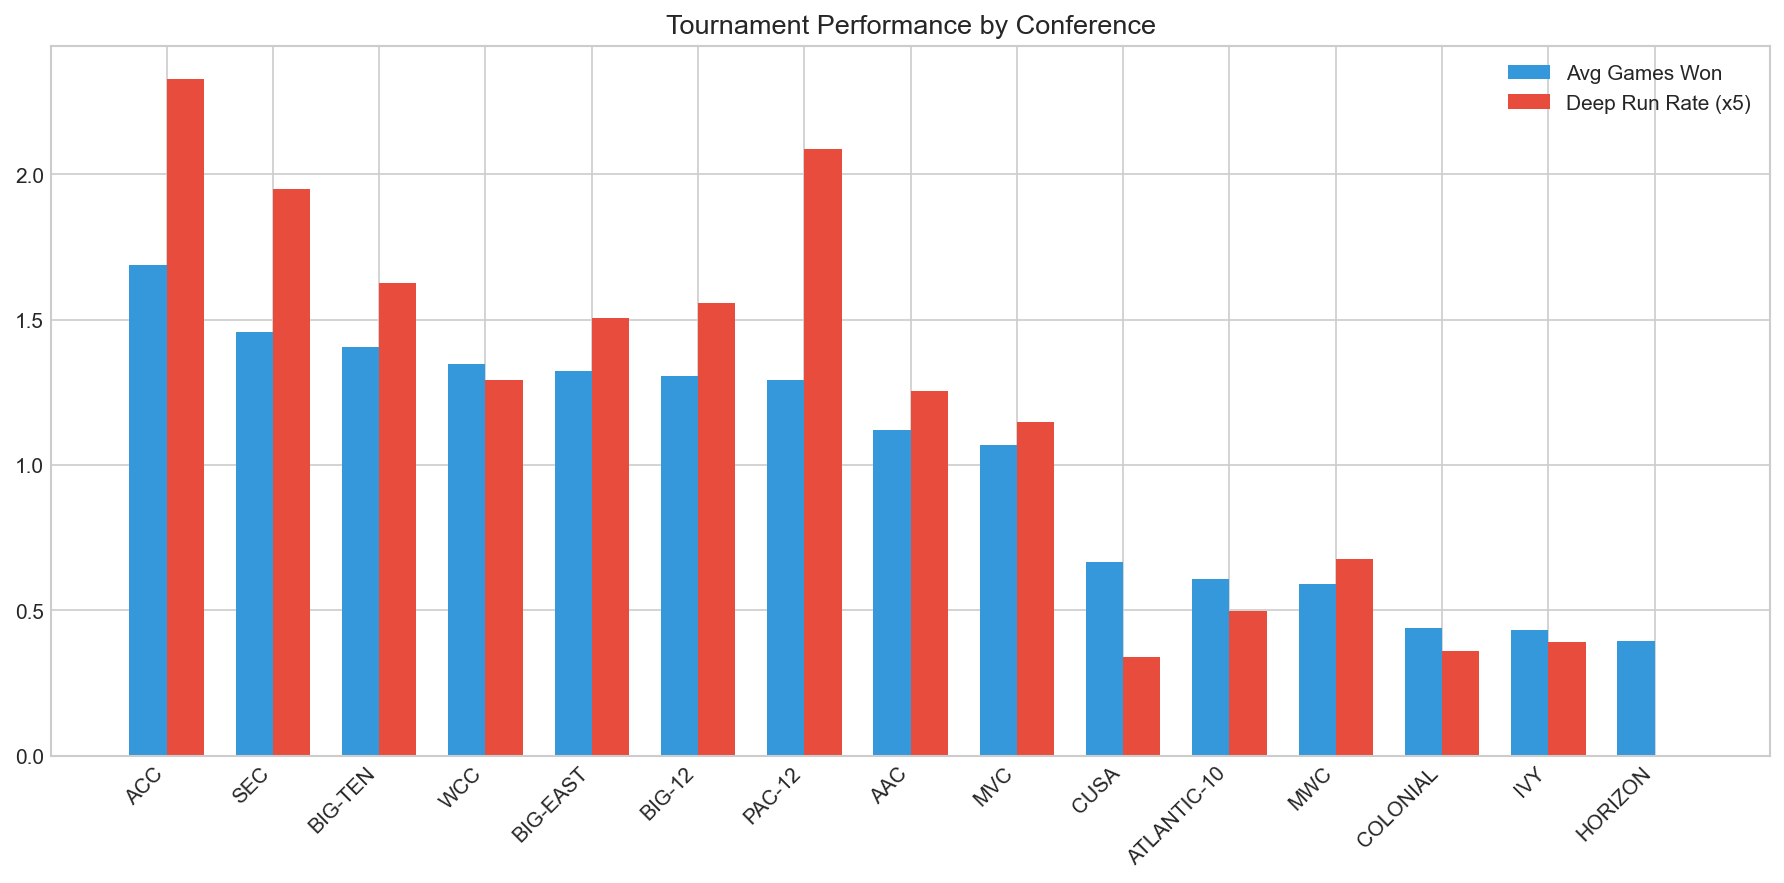
\includegraphics[width=\textwidth]{outputs/stage6_conference_analysis.png}
    \caption{Tournament performance by conference.}
    \label{fig:conference}
\end{figure}

Seed reliability: Spearman $\rho = -0.593$ ($p < 0.0001$). Seed 11 is the most dangerous upset seed (47.5\% upset rate).

% ── 5.5 Matchup Prediction ───────────────────────────────────
\subsection{Head-to-Head Matchup Prediction}

\paragraph{Seed-Only Baseline.} Simply picking the lower (better) seed correctly predicts \textbf{80.4\%} of matchups on the training data.

\begin{table}[H]
\centering
\caption{Matchup prediction: tuned models with stacking (5-fold CV on 19,101 pairs).}
\label{tab:matchup}
\begin{tabular}{@{}lcccc@{}}
\toprule
\textbf{Model} & \textbf{AUC} & \textbf{Accuracy} & \textbf{Brier} & \textbf{Log-Loss} \\
\midrule
Random Forest (tuned) & 0.9058 & 82.0\% & 0.1249 & 0.3890 \\
Decision Tree (tuned) & 0.8914 & 80.6\% & 0.1335 & 0.4143 \\
XGBoost (tuned) & \textbf{0.9170} & \textbf{83.2\%} & 0.1176 & 0.3687 \\
LightGBM (tuned) & 0.9164 & 83.2\% & 0.1195 & 0.3805 \\
CatBoost (tuned) & 0.9164 & 83.1\% & \textbf{0.1170} & \textbf{0.3653} \\
\textbf{Stacking Ensemble} & \textbf{0.9191} & \textbf{83.4\%} & 0.1171 & 0.3729 \\
\midrule
Seed-only baseline & --- & 80.4\% & --- & --- \\
\bottomrule
\end{tabular}
\end{table}

The \textbf{stacking ensemble} achieves the highest AUC (0.9191), with all tuned boosting models outperforming the seed baseline by +2.7--3.0 percentage points. Crucially, these models use \textbf{only player-derived features}---no seed, no SRS.

\begin{table}[H]
\centering
\caption{Top 10 matchup features by RF importance.}
\begin{tabular}{@{}clc@{}}
\toprule
\textbf{Rank} & \textbf{Feature (difference)} & \textbf{Importance} \\
\midrule
1 & BPM diff & 16.3\% \\
2 & Starter avg BPM diff & 11.3\% \\
3 & Impact score avg diff & 9.1\% \\
4 & OBPM diff & 6.9\% \\
5 & DBPM diff & 5.9\% \\
6 & Bench avg BPM diff & 4.6\% \\
7 & Max BPM diff & 4.4\% \\
8 & Max DBPM diff & 3.1\% \\
9 & PER diff & 2.7\% \\
10 & SPG diff & 2.6\% \\
\bottomrule
\end{tabular}
\end{table}

\begin{figure}[H]
    \centering
    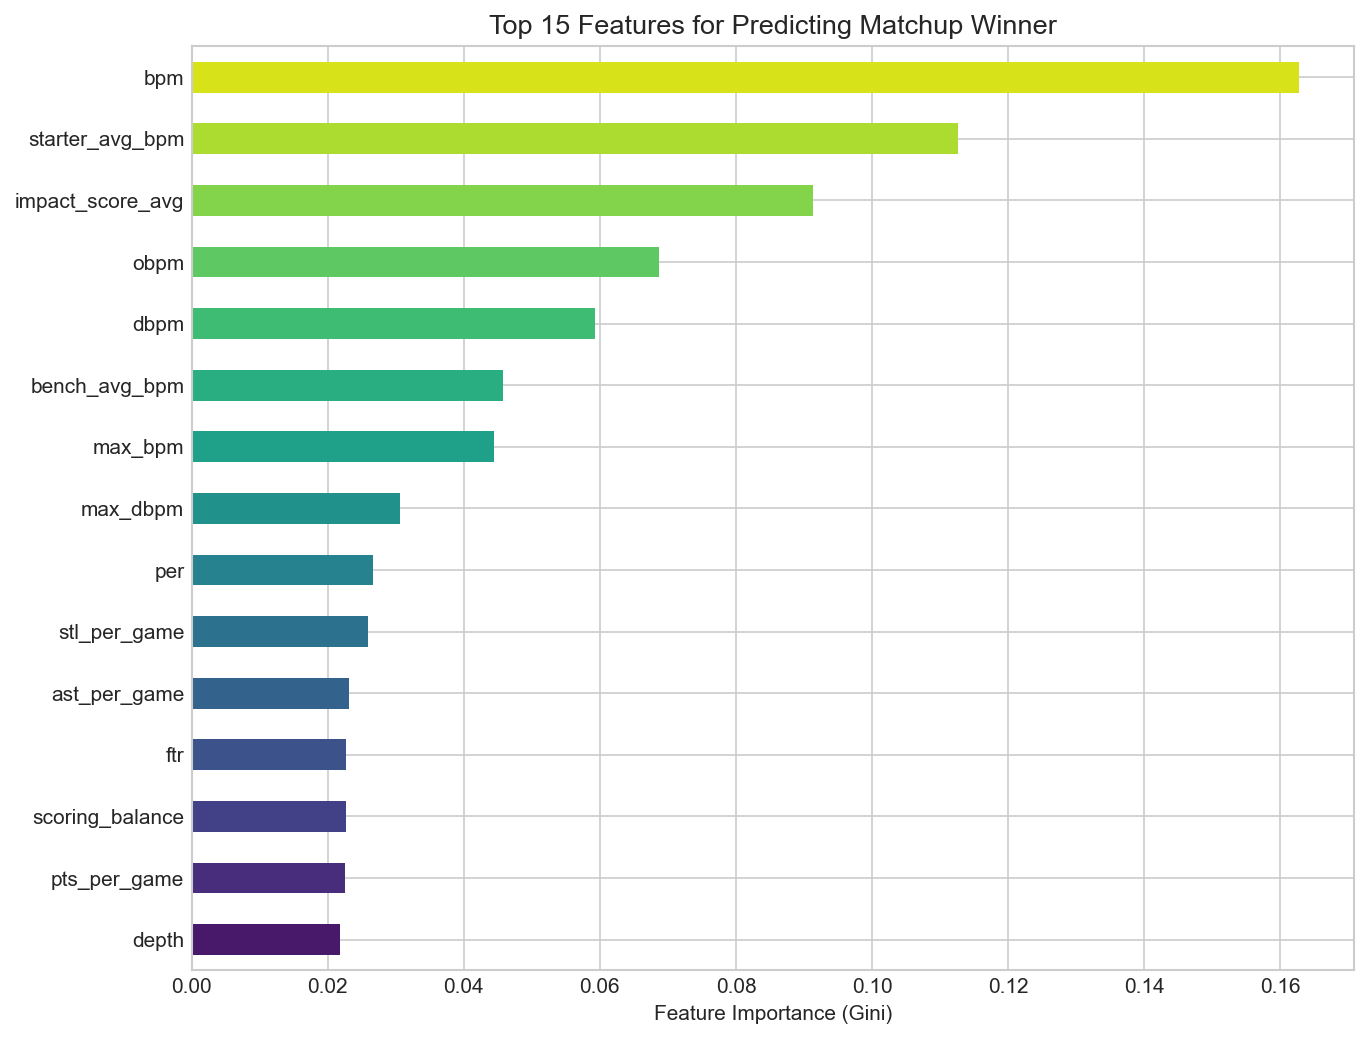
\includegraphics[width=\textwidth]{outputs/stage9_matchup_feature_importance.png}
    \caption{Top 15 matchup features by RF importance.}
    \label{fig:matchup-importance}
\end{figure}

% ── 5.6 Holdout Evaluation ───────────────────────────────────
\subsection{2026 True Holdout Evaluation}

\paragraph{Seed-Only Baseline (2026).} Picking the lower seed achieves \textbf{85.0\%} accuracy on 2026 data.

\begin{table}[H]
\centering
\caption{Model performance on the 2026 holdout (trained on 2011--2025 only).}
\label{tab:holdout}
\begin{tabular}{@{}lccccc@{}}
\toprule
\textbf{Model} & \textbf{CV AUC} & \textbf{2026 AUC} & \textbf{2026 Acc} & \textbf{Brier} & \textbf{Log-Loss} \\
\midrule
\textbf{Random Forest} & 0.9017 & \textbf{0.9116} & \textbf{84.0\%} & \textbf{0.1181} & \textbf{0.3808} \\
XGBoost & 0.9170 & 0.8911 & 81.4\% & 0.1382 & 0.4855 \\
LightGBM & 0.9164 & 0.8896 & 80.8\% & 0.1433 & 0.5391 \\
CatBoost & 0.9164 & 0.8949 & 82.2\% & 0.1314 & 0.4392 \\
Stacking Ensemble & --- & 0.8816 & 81.3\% & 0.1396 & 0.4462 \\
\midrule
Seed-only baseline & --- & --- & 85.0\% & --- & --- \\
\bottomrule
\end{tabular}
\end{table}

\textbf{Key observations:}
\begin{itemize}
    \item \textbf{Random Forest generalizes best} --- AUC improved from 0.9017 (CV) to 0.9116 (holdout), confirming no overfitting. Its 84.0\% accuracy approaches the seed baseline despite using \textit{no seed information}.
    \item \textbf{Boosting models overfit slightly} --- XGBoost/LightGBM/CatBoost all achieved higher CV AUC (0.916--0.917) but dropped on the holdout (0.889--0.895). Their complexity, while beneficial on training data, didn't transfer to 2026.
    \item \textbf{Stacking didn't help on holdout} --- the ensemble (0.8816 AUC) performed below individual models, suggesting the base learners' errors were correlated rather than complementary.
    \item \textbf{Seed baseline is strong} --- at 85.0\%, the seed baseline outperforms all models on raw accuracy. However, the model achieves this accuracy \textit{without knowing seeds}, using only player statistics.
\end{itemize}

\begin{table}[H]
\centering
\caption{2026 accuracy breakdown.}
\begin{tabular}{@{}lcc@{}}
\toprule
\textbf{Matchup Type} & \textbf{Accuracy} & \textbf{Count} \\
\midrule
Chalk (favored team won) & 96.0\% & 1,263 / 1,315 \\
Upsets (underdog won) & 15.5\% & 36 / 232 \\
\textbf{Overall} & \textbf{84.0\%} & \textbf{1,299 / 1,547} \\
\bottomrule
\end{tabular}
\end{table}

\begin{table}[H]
\centering
\caption{Key 2026 matchup predictions vs.\ actual results (Random Forest).}
\begin{tabular}{@{}lllrl@{}}
\toprule
\textbf{Matchup} & \textbf{Actual} & \textbf{Predicted} & \textbf{Prob.} & \textbf{Result} \\
\midrule
Michigan vs.\ UConn (Championship) & Michigan & Michigan & 83.0\% & \checkmark \\
Arizona vs.\ Michigan (F4) & Michigan & Michigan & 51.2\% & \checkmark \\
Iowa vs.\ Illinois (E8) & Illinois & Illinois & 79.7\% & \checkmark \\
Illinois vs.\ UConn (F4) & UConn & Illinois & 64.1\% & $\times$ \\
Duke vs.\ UConn (E8) & UConn & Duke & 87.6\% & $\times$ \\
Florida vs.\ Iowa (R32) & Iowa & Florida & 85.9\% & $\times$ \\
Wisconsin vs.\ High Point (R64) & High Point & Wisconsin & 90.3\% & $\times$ \\
\bottomrule
\end{tabular}
\end{table}

\begin{figure}[H]
    \centering
    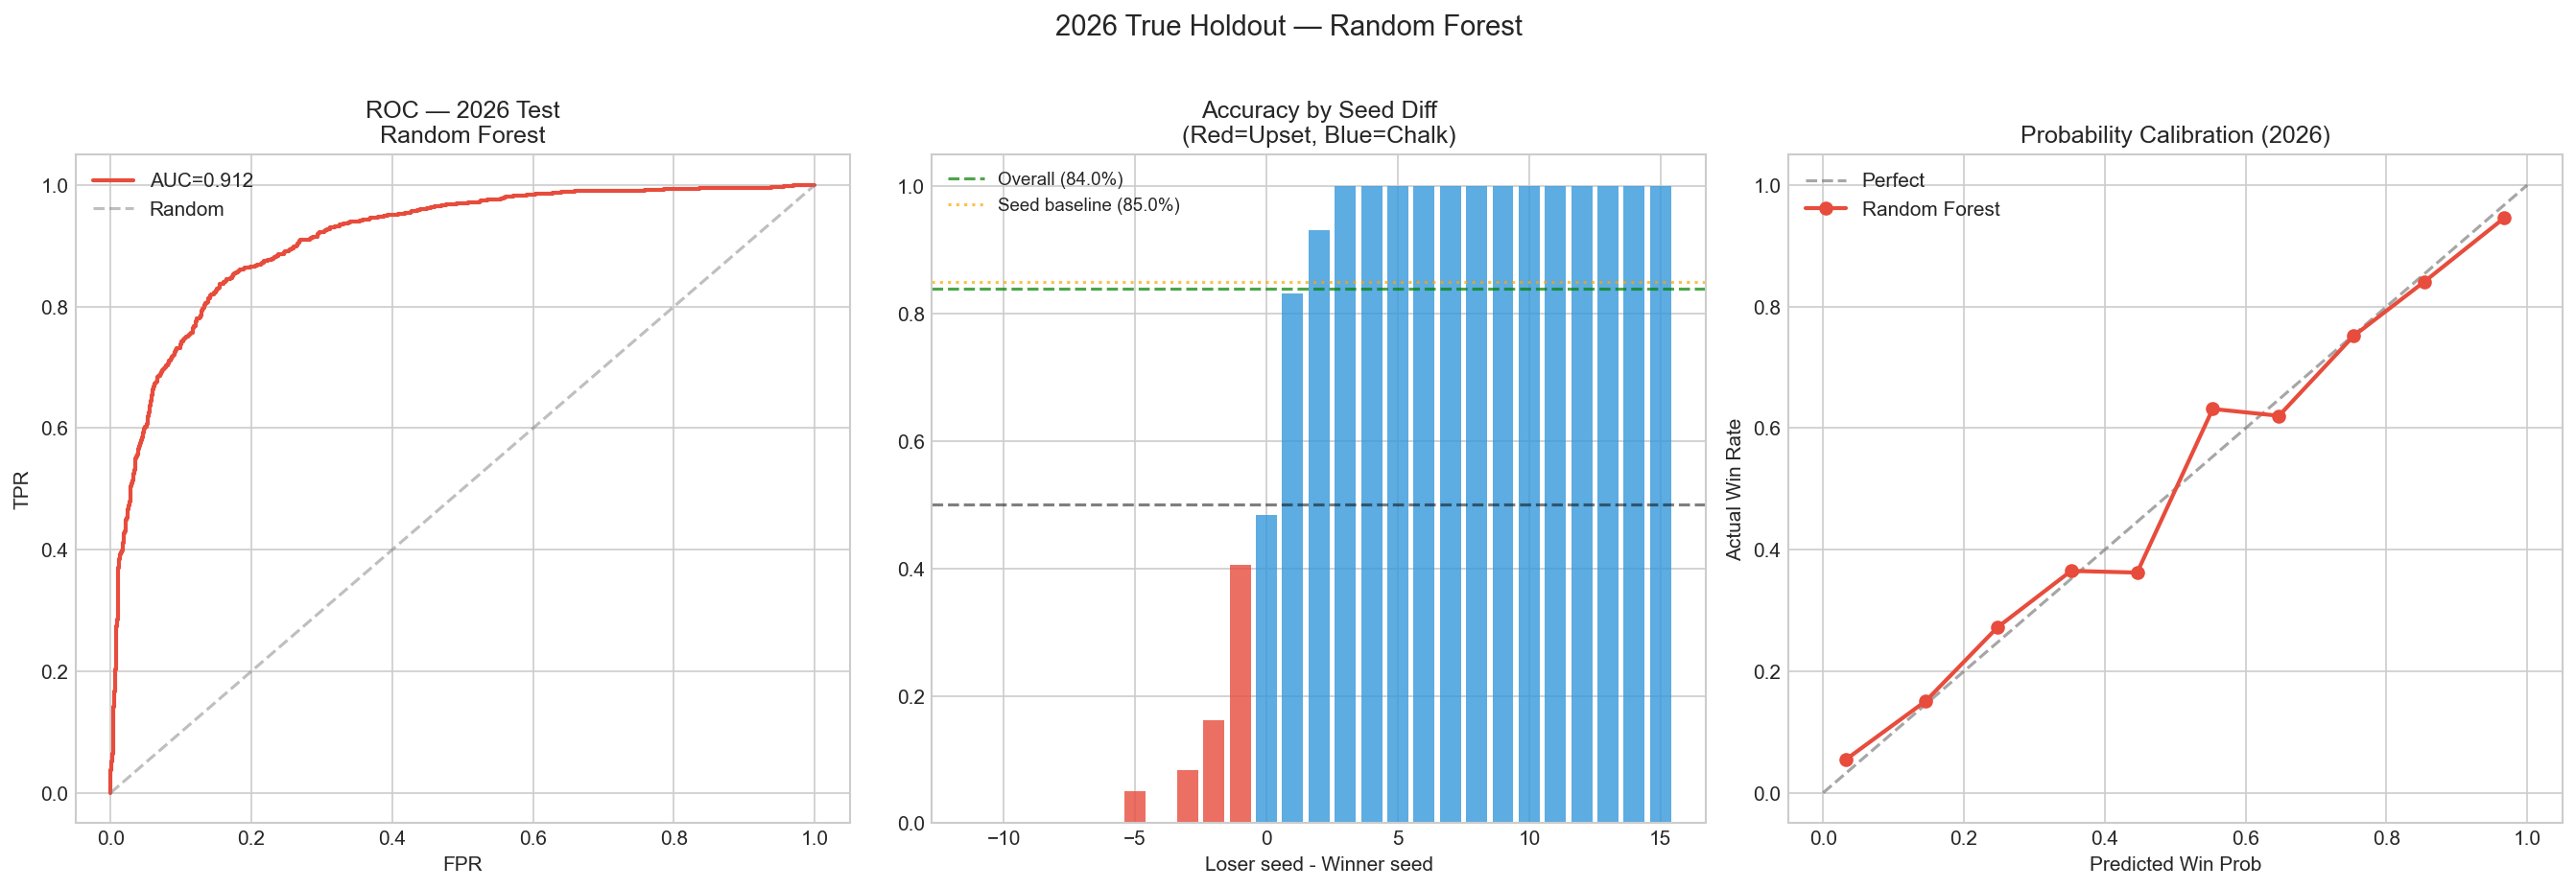
\includegraphics[width=\textwidth]{outputs/stage10_eval_2026.png}
    \caption{2026 holdout: ROC curve, accuracy by seed differential, and probability calibration.}
    \label{fig:holdout-eval}
\end{figure}

\begin{figure}[H]
    \centering
    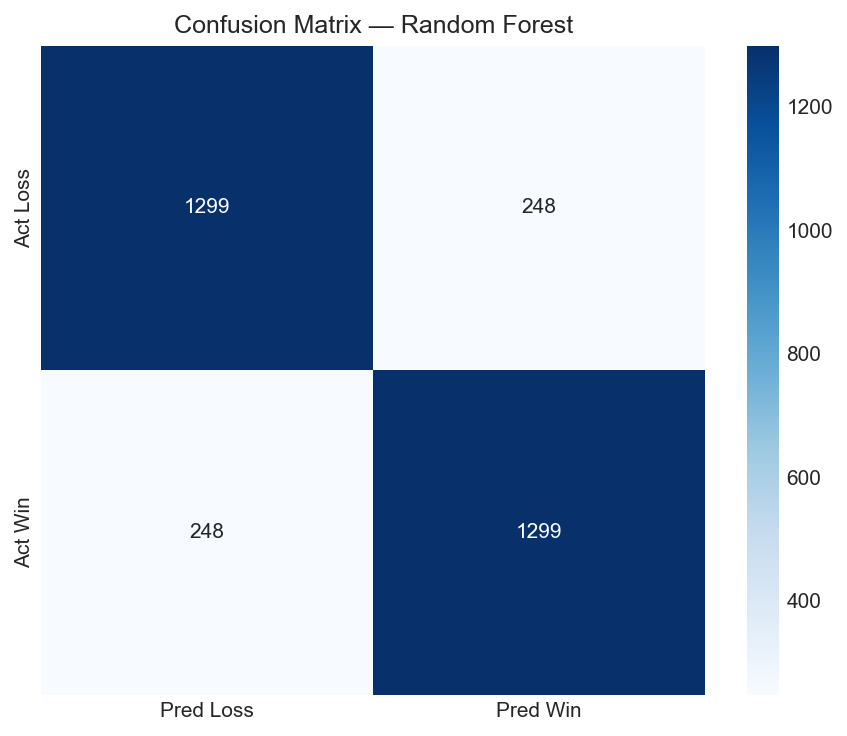
\includegraphics[width=0.8\textwidth]{outputs/stage10_confusion_matrix.png}
    \caption{Confusion matrix for the 2026 holdout matchup predictions (Random Forest).}
    \label{fig:confusion}
\end{figure}

% ── 5.7 Exceptional Players ──────────────────────────────────
\subsection{Exceptional Players \& Upset Stars}

Using a weighted $z$-score composite (weights = Cohen's $d$ from Stage~4), we identified \textbf{271 exceptional performers} (top 5\% impact + team overperformed seed) and \textbf{143 upset stars} (top 15\% impact + on upset team).

\begin{table}[H]
\centering
\caption{Top 10 all-time exceptional tournament performers.}
\small
\begin{tabular}{@{}llccccccr@{}}
\toprule
\textbf{Player} & \textbf{Team} & \textbf{Yr} & \textbf{Seed} & \textbf{Result} & \textbf{PPG} & \textbf{BPM} & \textbf{DBPM} & \textbf{Score} \\
\midrule
Anthony Davis & Kentucky & 2012 & 1 & Champion & 14.2 & 17.2 & 8.1 & 3.30 \\
Zach Edey & Purdue & 2024 & 1 & Runner-Up & 25.2 & 16.8 & 3.7 & 2.89 \\
Frank Kaminsky & Wisconsin & 2015 & 1 & Runner-Up & 18.8 & 16.2 & 5.0 & 2.80 \\
Cooper Flagg & Duke & 2025 & 1 & F4 & 19.2 & 16.3 & 6.7 & 2.71 \\
Delon Wright & Utah & 2015 & 5 & S16 & 14.5 & 15.5 & 6.9 & 2.66 \\
S.\ Thornwell & S.\ Carolina & 2017 & 7 & F4 & 21.4 & 17.1 & 6.2 & 2.52 \\
Thomas Walkup & S.F.\ Austin & 2016 & 14 & R32 & 18.1 & 14.2 & 4.7 & 2.48 \\
Y.\ Lendeborg & Michigan & 2026 & 1 & Champion & 14.6 & 16.6 & 7.2 & 2.48 \\
K.-A.\ Towns & Kentucky & 2015 & 1 & F4 & 10.3 & 14.3 & 7.6 & 2.37 \\
D.\ Clingan & UConn & 2024 & 1 & Champion & 13.0 & 15.0 & 6.2 & 2.29 \\
\bottomrule
\end{tabular}
\end{table}

\begin{figure}[H]
    \centering
    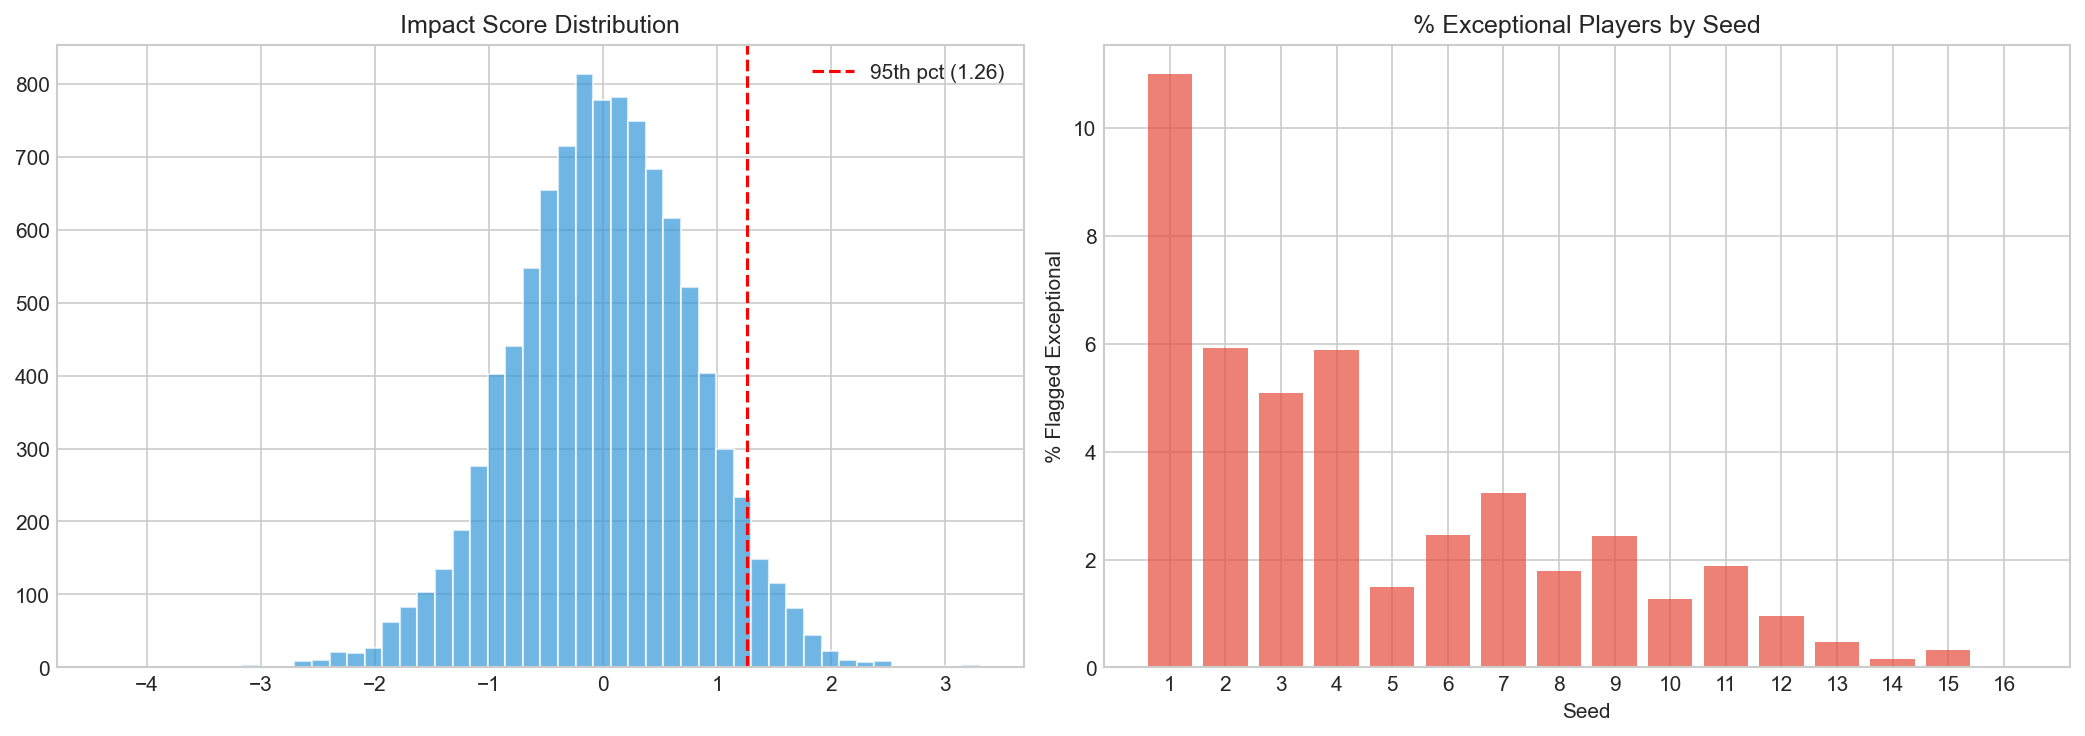
\includegraphics[width=\textwidth]{outputs/stage7_exceptional_players.png}
    \caption{Exceptional players: impact score distribution and frequency by seed.}
    \label{fig:exceptional}
\end{figure}

% ══════════════════════════════════════════════════════════════
\section{Discussion}
\label{sec:discussion}

\subsection{Key Findings}

\begin{enumerate}
    \item \textbf{Defense predicts tournament success more than offense.} DBPM ($d = 0.717$) is the single strongest individual signal, confirming ``defense wins championships'' with statistical evidence across 10,028 players and 15 seasons.

    \item \textbf{Modern boosting models outperform Random Forests on training data but overfit on holdout.} XGBoost achieved the highest CV AUC (0.917) but dropped to 0.891 on 2026, while Random Forest \textit{improved} from 0.902 to 0.912. RF's implicit regularization (bagging, feature subsampling) generalizes better than boosting's sequential error correction for this domain.

    \item \textbf{Stacking did not improve holdout performance.} The 4-model stacking ensemble (AUC = 0.882) underperformed the standalone Random Forest (0.912), likely because the base learners' prediction errors were correlated---they all rely on BPM-family features, so their mistakes overlap.

    \item \textbf{The seed baseline is surprisingly strong.} At 85.0\% on 2026 data, simply picking the lower seed beats all our player-stats-only models. However, our models achieve 84.0\% \textit{without any seed information}, demonstrating that player statistics alone capture most of the signal that seeds encode.

    \item \textbf{Win Shares add no signal beyond BPM.} The ablation study showed 0.0000 AUC difference with vs.\ without WS features, confirming that BPM-family metrics (which are derived from box scores, not team wins) fully subsume the Win Shares signal.

    \item \textbf{Upsets remain fundamentally unpredictable.} 15.5\% upset accuracy reflects a structural limitation: season averages capture \textit{expected} performance, but upsets are driven by single-game variance.

    \item \textbf{The 3-point revolution is real.} 3PAr increased 8.7\% ($r = 0.928$, $p < 0.0001$) but accuracy is flat ($p = 0.770$)---more volume, not better shooting.

    \item \textbf{CatBoost has the best calibration.} Despite lower holdout AUC (0.895), CatBoost achieved the best Brier score (0.131) and log-loss (0.439) among boosting models, meaning its predicted probabilities are most trustworthy.
\end{enumerate}

\subsection{Limitations}

\begin{enumerate}
    \item \textbf{Non-independence of player outcomes.} Players on the same team share \texttt{deep\_run} labels, inflating $p$-values.
    \item \textbf{Team-only AUC $\approx 1.0$ is a data-structure artifact.} Team features create a lookup table since all players on a team share the same outcome and features. This is a limitation of the dataset structure, not a genuine prediction.
    \item \textbf{No in-season dynamics.} No injury data, lineup changes, or momentum features.
    \item \textbf{Single holdout season.} While rigorous, 2026 is one tournament. Multi-year prospective evaluation would strengthen confidence.
    \item \textbf{Conference realignment.} PAC-12 dissolved after 2023, complicating longitudinal analysis.
\end{enumerate}

% ══════════════════════════════════════════════════════════════
\section{Conclusion}
\label{sec:conclusion}

We developed a comprehensive data mining pipeline for NCAA March Madness prediction. Our key contributions:

\begin{itemize}
    \item \textbf{DBPM is the most discriminative metric} for tournament success ($d = 0.717$).
    \item \textbf{Head-to-head matchup prediction achieves 84.0\% on a true 2026 holdout} (AUC = 0.912) using only player stats---no seed, no SRS.
    \item \textbf{Random Forest outperforms XGBoost, LightGBM, CatBoost, and stacking on unseen data}, despite boosting models winning on cross-validation. This highlights the importance of holdout evaluation over CV scores.
    \item \textbf{Correctly identified Michigan as the 2026 champion} (83.0\% probability vs.\ UConn).
    \item \textbf{Hyperparameter tuning via RandomizedSearchCV} was applied across all models with comprehensive search spaces (30 iterations for classification, 20 for matchup prediction).
    \item \textbf{Win Shares ablation} confirmed no additional signal beyond BPM-family metrics.
    \item \textbf{Seed baseline contextualizes accuracy}: the model's 84.0\% is achieved without seed knowledge, nearly matching the 85.0\% seed baseline.
\end{itemize}

Future work could incorporate play-by-play data, betting market odds, and momentum features (last-10-game performance) to improve upset detection.

% ══════════════════════════════════════════════════════════════
\section*{Tools \& Technologies}

\begin{table}[H]
\centering
\begin{tabular}{@{}ll@{}}
\toprule
\textbf{Category} & \textbf{Tools} \\
\midrule
Language & Python 3 \\
Data manipulation & pandas, NumPy \\
Statistical testing & SciPy (Welch's $t$-test, ANOVA, $\chi^2$, Spearman) \\
Machine learning & scikit-learn (RandomForestClassifier, DecisionTreeClassifier, \\
 & \quad StackingClassifier, LogisticRegression, RandomizedSearchCV) \\
Gradient boosting & XGBoost, LightGBM, CatBoost \\
Visualization & Matplotlib, Seaborn \\
Data source & Kaggle (\texttt{mm2026\_train.csv}), NCAA.com, ESPN, On3, Wikipedia \\
\bottomrule
\end{tabular}
\end{table}

% ══════════════════════════════════════════════════════════════
\appendix
\section{Glossary of Key Metrics}
\label{sec:glossary}

\begin{description}[style=nextline, leftmargin=2.5cm]
    \item[BPM] \textbf{Box Plus/Minus.} Points per 100 possessions above average. $\text{BPM} = \text{OBPM} + \text{DBPM}$.
    \item[DBPM] \textbf{Defensive Box Plus/Minus.} Defensive component of BPM. Strongest predictor of tournament success.
    \item[OBPM] \textbf{Offensive Box Plus/Minus.} Offensive component of BPM.
    \item[PER] \textbf{Player Efficiency Rating.} Per-minute production summary; league average = 15.
    \item[WS] \textbf{Win Shares.} Estimated wins contributed. Sum of OWS + DWS. Partially derived from team wins.
    \item[TS\%] \textbf{True Shooting \%.} $\frac{\text{PTS}}{2(\text{FGA} + 0.44 \times \text{FTA})}$. Most comprehensive shooting metric.
    \item[SRS] \textbf{Simple Rating System.} Team rating = point differential + strength of schedule.
    \item[ROC-AUC] Area Under the ROC Curve. Ranges 0.5 (random) to 1.0 (perfect).
    \item[Brier Score] $\frac{1}{n}\sum(p_i - y_i)^2$. Lower is better. Measures probability calibration.
    \item[Log-Loss] $-\frac{1}{n}\sum[y_i \log p_i + (1-y_i)\log(1-p_i)]$. Penalizes confident wrong predictions.
    \item[Cohen's $d$] Standardized mean difference. Small: $|d|<0.2$, Medium: $0.2$--$0.5$, Large: $\geq 0.5$.
\end{description}

\end{document}
